%% Template baseado no do Prof. Arnaldo Mandel
%% Veja https://www.ime.usp.br/~am/414/listas/index.html

\documentclass[12pt]{article}

%% Escrevendo em português:

%\usepackage[brazilian]{babel}
\usepackage[utf8]{inputenc}
%\usepackage{textcomp}
\usepackage[T1]{fontenc}
\usepackage{lmodern}
%----------------------------

\setlength{\topmargin}{-.5in}
\setlength{\textheight}{9in}
\setlength{\textwidth}{6.3in}
\setlength{\oddsidemargin}{-.125in}
\setlength{\evensidemargin}{-.125in}

\usepackage[usestackEOL]{stackengine}
\usepackage{xspace}
\usepackage{pifont}
\usepackage{amsmath}
\usepackage{amsfonts}
\usepackage[dvipsnames]{xcolor}
\usepackage{fancybox}
\usepackage{amsthm}
\usepackage{listings}
\usepackage{hyperref}
\usepackage{todonotes}

\usepackage{MnSymbol,wasysym}
\usepackage{marvosym}

\pagestyle{empty}

\definecolor{darkgreen}{RGB}{0, 133, 117}
\definecolor{yelloworange}{HTML}{FAA21A}

\newcommand{\N}{{\tt I\kern-.2em N \relax}}      % N        |N
\def\pule{\vspace{0.2cm}}
\def\pulao{\vspace{0.5cm}}
\def\pulaozao{\vspace{1cm}}
\def\ni{\noindent}

\newcommand{\Si}{\ensuremath{\Sigma}\xspace}
\newcommand{\Sis}{\ensuremath{\Sigma^*}\xspace}
\newcommand{\Ga}{\ensuremath{\Gamma}\xspace}
\newcommand{\Gas}{\ensuremath{\Gamma^*}\xspace}
\newcommand{\serio}{\ding{98}\xspace}
\newcommand{\LP}{L\&P\xspace}
\newcommand{\conj}[2]{\ensuremath{\{#1\,|\;#2\}}}
\DeclareMathOperator{\Ima}{Im}
\newcommand{\ssq}{\ensuremath{\subseteq}\xspace}
\newcommand{\union}{\mathop{\bigcup}\displaylimits}
\newcommand{\Rfield}[1]{\ensuremath{\mathbb{R}^{#1}}\xspace}
\newcommand{\del}{\ensuremath{\text{d}}\xspace}
\newcommand{\expct}[1]{\ensuremath{\langle {#1} \rangle}\xspace}

\begin{document}

\newtheorem{theorem}{Teorema}%[section]
\newtheorem{corollary}{Corolário}[theorem]
\newtheorem{lemma}[theorem]{Lema}

\begin{center}
\Huge \bf
Automatic Detection of Parallelization Viability
\vspace{0.5cm}
\end{center}
\vspace*{\fill}
{
     \centering
     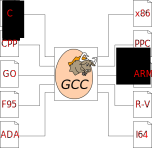
\includegraphics[scale=0.7]{logo.pdf}
    \par
}
\vspace*{\fill}
\normalsize{
\noindent\textcolor{darkgreen}{Giuliano Belinassi} \\
Timezone: GMT$-$3:00 \\
University of São Paulo -- Brazil \\
IRC: giulianob in \#gcc \\
Email: \href{mailto:giuliano.belinassi@usp.br}{\texttt{giuliano.belinassi@usp.br}} \\
Github: \url{https://github.com/giulianobelinassi/} \\
Date: \today
}
\newpage

\begin{section}{About Me}
    Computer Science Bachelor (University of São Paulo),
    currently pursuing a Masters Degree in Computer Science at the same
    institution. I've always been fascinated by topics such as
    High-Performance Computing and Code Optimization, having worked with
    a parallel implementation of a Boundary Elements Method software in GPU.
    I am currently conducting research on compiler parallelization and
    developing the \href{https://gcc.gnu.org/wiki/ParallelGcc}{ParallelGcc} project,
    having already presented it in \href{https://www.youtube.com/watch?v=jd6R3IK\_\_1Q}{GNU Cauldron 2019}.

    \textbf{Skills}: Strong knowledge in C, Concurrency, Shared Memory Parallelism, Multithreaded Debugging and other typical programming tools.
\end{section}

\begin{section}{Brief Introduction}

In ParallelGcc, we showed that parallelizing the Intra Procedural optimizations
improves speed when compiling huge files by a factor of 1.8x in a 4 cores
machine. There, the compilation were parallelized with threads, and due to
concurrency issues, it is still not merged into the main branch.

In this project, however, we plan to use the LTO infrastructure to improve
compilation performance, with a tradeoff of generating a binary as good as
if LTO is disabled.

\begin{subsection}{Modification to LTO}

The Link Time Optimization (LTO) is a compilation technique that allows the
compiler to analyse the program as a whole, instead of analysing and compiling
one file at time. Therefore, LTO is able to collect more information about
the program and generate a better optimization plan. LTO is divided in three
parts:

\begin{itemize}
    \item \emph{LGEN (Local Generation)}: Each file is translated to GIMPLE. This
        stage runs in parallel in each file.

    \item \emph{WPA (Whole Program Analysis)}: Run the Inter Procedural Analysis (IPA) in the
        entire program. This state runs serially.

    \item \emph{LTRANS (Local Transformation)}: Execute all Intra Procedural Optimizations in
        each partition. This stage runs in parallel.
\end{itemize}

The main issue here is that WPA can bottleneck the compilation in a many-core
machine because this runs serially, and therefore it can not take advantage of
all these extra cores. In this project, we aim to run the WPA stage in parallel
to each file, just like it is done when LTO is disabled. The advantage of doing
this way is that:

\begin{itemize}

    \item It can generate binaries as good as when LTO is disabled.
    \item It is faster, as we can partition big files into multiple partitions
    and compile these partitions in parallel
    \item It can interact with GNU Make Jobserver, improving CPU utilization.

\end{itemize}

\end{subsection}

\begin{subsection}{Planned Tasks}

I plan to use the GSoC time to develop the following topics:

\begin{itemize}
 \item{Week [1, 3] -- April 27 to May 15:} \\

  Update cc1, cc1plus, f771, ..., to partition the data after IPA
  analysis directly into multiple LTRANS partitions, instead of
  generating a temporary GIMPLE file.


 \item{Week [4, 7] -- May 18 to June 12:} \\

  Update the 'gcc' driver to take these multiple LTRANS partitions,
  then call the compiler and assembler for each of them, and merge into
  one object file. I might use the LTO LTRANS object streaming, therefore
  it should interact with GNU Make Jobserver.

 \item{Week 8 -- June 15 to 19:} \textbf{First Evaluation} \\

  Deliver a non-optimized version of the project. Here, it should
  be compiling some programs correctly, but probably there will be
  a huge overhead because so far there should not be any criteria
  about when to partitionate. Some tests are also planned for this
  evaluation.

 \item{Week [9, 11] -- June 22 to July 10:} \\

  Implement a criteria about when to partition, and interactively
  improve it based on data.

 \item{Week 12 --- July 13 to 17:} \textbf{Second Evaluation} \\

  Deliver a more optimized version of the project. Here we should
  filter files that would compile fast from files that would require
  partitioning, and therefore we should see some speedup.

\item{Week [13, 15] --- July 20 to August 10:} \\

  Develop more tests to this feature, and address unexpected issues
  so that this feature can be merged to trunk for the next GCC
  release.

\item{Week 16:} \textbf{Final evaluation}\\
  Deliver the final product as a series of patches for trunk.


\end{itemize}
\end{subsection}

\end{section}
\end{document}
